
	\chapter{Merging similar operators -mo}
	
	Let assume that we have two or more actions that are similar (\ref{notation:similarActions}). In such case we can select only one action and the rest remove. This is because rest of the actions become redundant. By this, number of action is decreased and some other reduction may start to work because we get rid of multiple possibilities how to add some fact (some reductions need to know that the fact is added only by one action, etc).
	
	\begin{figure}
		\begin{subfigure}[b]{0.4\textwidth}
			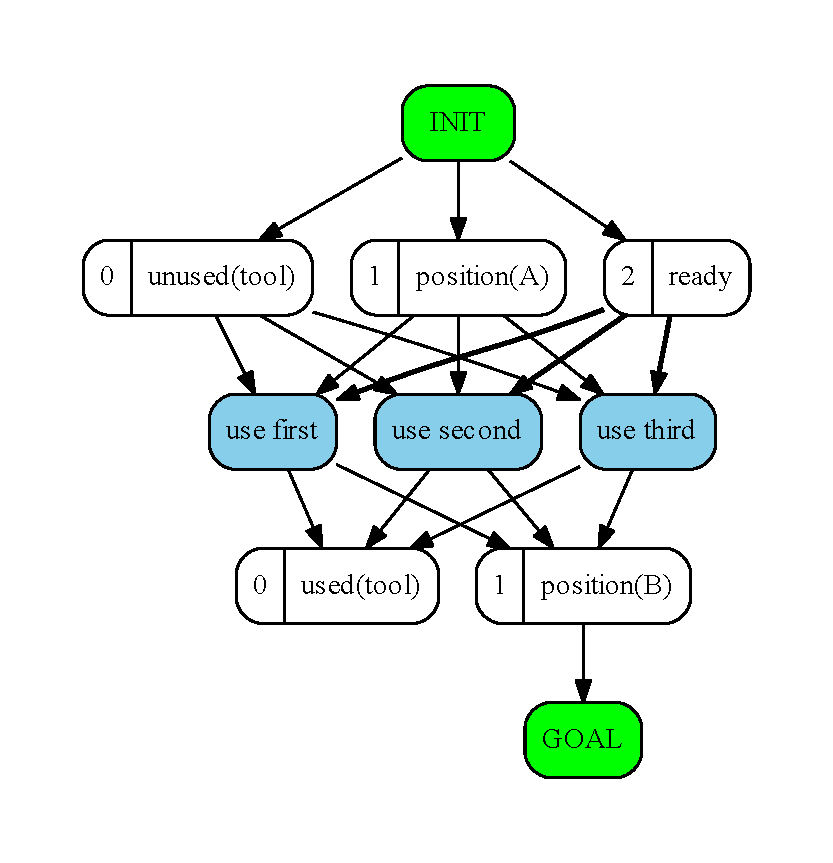
\includegraphics[scale=0.4]{mergingSimilarOperators/figures/threeToOne_input}
			\caption{before reduction}
		\end{subfigure}	
		\begin{subfigure}[b]{0.4\textwidth}
			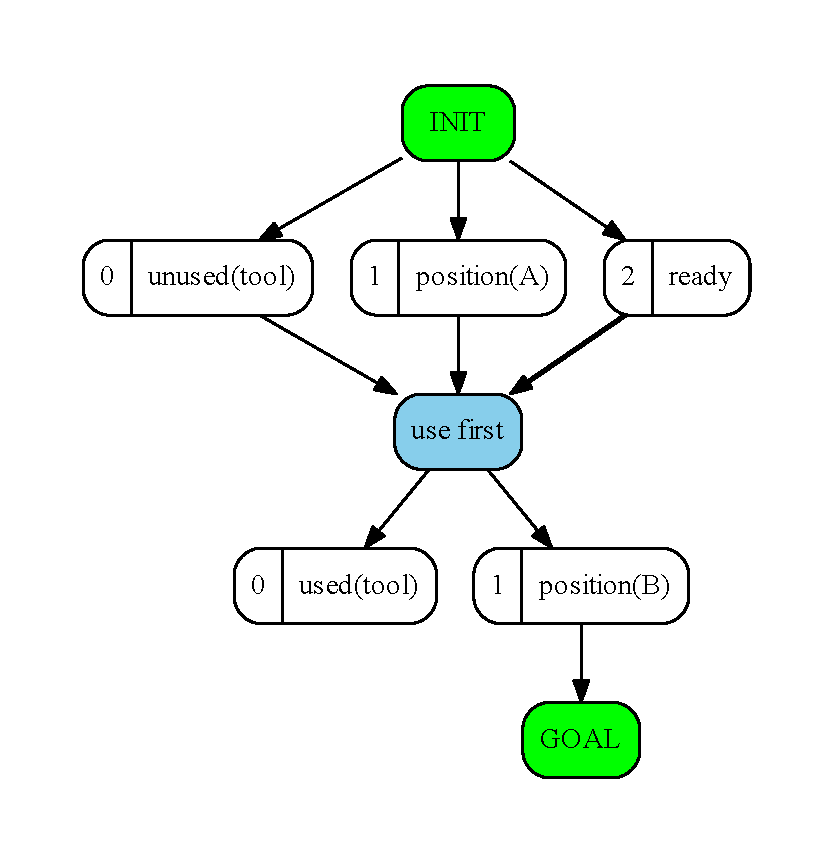
\includegraphics[scale=0.4]{mergingSimilarOperators/figures/threeToOne_output}
			\caption{after reduction}
		\end{subfigure}
		\caption{All of the action in the example can be removed, but one representative of these action has te be preserved in the instance.}		
	\end{figure}	
	
	
	\section{Reduce operation}
	Let's have SAS in form $<\vars, \init, \goal, \actions, \mutexes{}>$. The following reductions is executed only if there is a set of similar actions that has got more than one action. Let have such a set $\actions{}_s$.
	
	The reduction does following things: pick arbitrary action $a \in \actions{}_s$. Remove all actions from $\actions{}$ each action in $\actions{}_s$ but not $a$; $\actions{}' \leftarrow (\actions \setminus \actions{}_s) \cup \{a\}$.
	
	Output of the reduction is SAS $<\vars{}, \init{}, \goal{}, \actions{}', \mutexes{}>$.
	
	\section{Possible outgoing states of SAS}
	\begin{enumerate}
		\item possible state of SAS for application of -sd
	\end{enumerate}
	
	\section{States before application of this operation}
	\begin{itemize}
		\item original SAS
		\item after -dv, -mv, -oe
	\end{itemize}
	
	
	\section{Reverse operation}
	Since the actions have got same effects and preconditions, only $a$ is allowed to be used in the plan. Moreover, no extending of the plan is done. This comes from the fact that we think that if two actions are similar, then they were either similar from the start or they got similar during reductions. If they got similar during reductions, then we can get by application of reverse operators from one action to another (in the similar set), eg. to get to state where any of the action from the $\actions{}_s$ is applicable. But this is rather unproven idea.
	
	\section{Implementation notes}
	There could be (but is not implemented) filter for deleting similar actions while parsing. Because then we would have the information whether the actions were similar from the beginning or if they become similar during reductions.
	
	
	
	